\documentclass[10pt,a4paper]{labreport}
\usepackage{csquotes}
\usepackage{titlesec}
\usepackage{ragged2e}
\usepackage{siunitx}
\usepackage{setspace}
\usepackage{longtable}
\usepackage{rotating}
\usepackage{xurl}
\usepackage{physics}
\usepackage{caption}
\usepackage{wrapfig}
\usepackage{tabularray}
\usepackage{fancyhdr}
\usepackage{subcaption}
\usepackage{lscape}
\usepackage{tensor}
\usepackage{multirow}
\usepackage[gen]{eurosym}
\usepackage{float}
\usepackage{bm}
\usepackage{lipsum}
\usepackage{parskip}
\usepackage{booktabs}
\usepackage{enumerate}
\usepackage[justification=justified]{caption}
\usepackage[nottoc]{tocbibind}
\usepackage{hyperref}
   \usepackage[
  backend=biber,
  style=chem-acs,articletitle=true,doi=true]{biblatex}
  \addbibresource{references.bib}
\usepackage{color}

\usepackage{listings}
\definecolor{codegreen}{rgb}{0,0.6,0}
\definecolor{codegray}{rgb}{0.5,0.5,0.5}
\definecolor{codepurple}{rgb}{0.58,0,0.82}
\definecolor{backcolour}{rgb}{0.95,0.95,0.92}
\lstdefinestyle{mystyle}{
    backgroundcolor=\color{backcolour},   
    commentstyle=\color{codegreen},
    keywordstyle=\color{codepurple},
    numberstyle=\tiny\color{codegray},
   % stringstyle=\color{grey},
    basicstyle=\ttfamily\footnotesize,
    breakatwhitespace=false,         
    breaklines=true,                 
    captionpos=b,                    
    keepspaces=true,                 
    numbers=left,                    
    numbersep=5pt,                  
    showspaces=false,                
    showstringspaces=false,
    showtabs=false,                  
    tabsize=5
}
\lstset{style=mystyle}




\title{Nanoscale Material Modelling
\\
\normalsize{Week 6}} % Main title and sub title. 

\author{Ilija A. Gjerapić, S4437586; \href{mailto:i.a.gjerapic@student.rug.nl}{i.a.gjerapic@student.rug.nl}; \href{https://github.com/igjerapic/nmm-week6/}{@github} } % Name, student number, email

\supervisors{prof. dr. A. Giuntoli, prof. dr. J. Slawinska}

\begin{document}


\maketitle
\tableofcontents


  

\thispagestyle{firststyle}
\newpage
\section{Assignment 1: Who needs Atoms?}
\subsection{All Atom Model Information}  
  Figure \ref{fig:ass1_PLA} shows the \texttt{Ovito} visualization of the \texttt{PLA\_CHARMM.data} file. Using the \texttt{Expresssion Selection} of the \texttt{MoleculeIdentifier} property resulting in a single monomer containing nine atoms: two oxygens, four hydrogens, and three carbon atoms. 
  The polylatic acid was determined to made up of 50 monomers based on the number of carbons bounded to two oxygens. This method also includes the two monomers at the end, which consist of ten atoms each. Therefore, the entire system consists of 452 atoms.   
  \begin{figure}[h]
    \centering 
    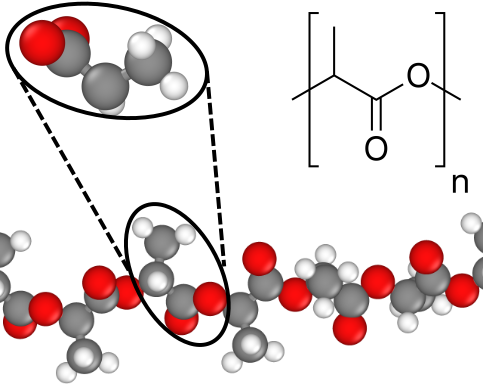
\includegraphics[width = 0.5\textwidth]{figs/ass1_PLA.png}
    \caption{An \texttt{Ovito} snapshot of the all-atom model of polylatic acid with an isolated monomer in the middle of the chain shown. Hydrogen atoms are white, oxygen atoms red, and carbon atoms grey. The chemical structure is also shown for reference.}
    \label{fig:ass1_PLA}
  \end{figure}

  \subsection{Defining Bonded Interactions of CG Model}

  To determine the bonded interactions of polylatic acid, the Boltzmann distribution of the energy
  \begin{equation}
    P(\epsilon_i) \propto \exp\left(-\frac{\epsilon_i}{k_B T}\right)
    \label{eq:Boltzmann}
  \end{equation} 
  for the bond distance, bond angle, and dihedral are fitted against their respective distributions collected during equilibrium. 
  Figure \ref{fig:ass1_equilib} demonstrates that equilibrium was reached prior to running the production run from which the bond distance, angle and dihedral distributions were determined.  
  \begin{figure}[h]
    \centering 
    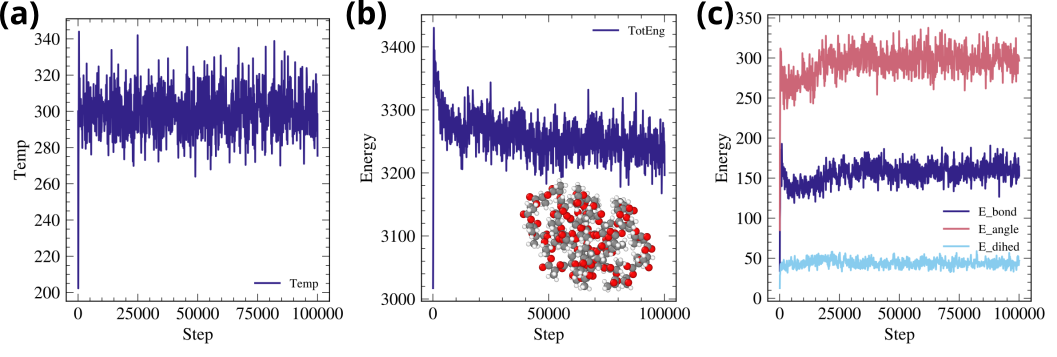
\includegraphics[width = 0.9\textwidth]{figs/ass1_equilib.png}
    \caption{The development of several thermodynamic properties during the equilibration run of polylatic acid. \textbf{(a)} shows the temperature, \textbf{(b)} the total energy, and \textbf{(c)} the bond-length, bond-angle, and dihedral energies. The inset in \textbf{(b)} shows an example configuration in equilibrium. }
    \label{fig:ass1_equilib}
  \end{figure}

  The bonded interactions between monomers were separated into contributions from the bond-length $r$, bond angle $\theta$ and dihedral angle $\phi$.
  The contribution from the bond-length between monomers was fitted against the \texttt{class2} bond style of LAMMPS
  \begin{equation}
    E_\text{bond} = K_{r,2}(r - r_0)^2 +   K_{r,3}(r - r_0)^3 +  K_{r,4}(r - r_0)^4,
    \label{eq:ass1_bondEngery}
  \end{equation}
  where $K_{r,i}$ are coefficients describing the strength of each term while $r_0$ is the minimum engery bond length. 
  Similarly, the bond angle between two CG beads was modelled as the \texttt{quartic} angle style:
    \begin{equation}
    E_\text{angle} = K_{\theta,2}(\theta - \theta_0)^2 +   K_{\theta,3}(\theta - \theta_0)^3 +  K_{\theta,4}(\theta - \theta_0)^4,
    \label{eq:ass1_angleEngery}
  \end{equation}
  where $\theta_0$ is the bond angle of minimum energy and $K_{\theta,i}$ coefficients describing the contribution of term. 
  Finally, the dihedral interaction between monomers was modelled as a sum of seven harmonics:
  \begin{equation}
    E_\text{dihed} = \sum_{i=1}^7 A_i \cos^{i-1}(\phi),
    \label{eq:ass1_dihedEnergy}
  \end{equation}

  The actual CG beads were defined as the center of masses of each monomer, which was achieved using \texttt{residues} of the simulation.
  
  \begin{lstlisting}[language=Python, 
    caption={An example on how the CG beads are defined from the all-atom simulation. The example is used when determining the bond lengths of the CG model.},
    label=lst:ass1_residues,
    ]
  bond_lengths = []
    residues = u.residues
    for ts in u.trajectory[start:end]:
        for i in range(1, len(residues) - 1):
            res1 = residues[i]
            res2 = residues[i + 1]
            com1 = res1.atoms.center_of_mass(unwrap=True)
            com2 = res2.atoms.center_of_mass(unwrap=True)
            bond = calc_bonds(com1[np.newaxis, :], com2[np.newaxis, :], 
                              box=u.dimensions)[0]
            bond_lengths.append(bond)
    return bond_lengths
  \end{lstlisting}
  \subsection{Distribution of Bonds, Angles, and Dihedrals}
  \begin{figure}[h]
    \centering 
    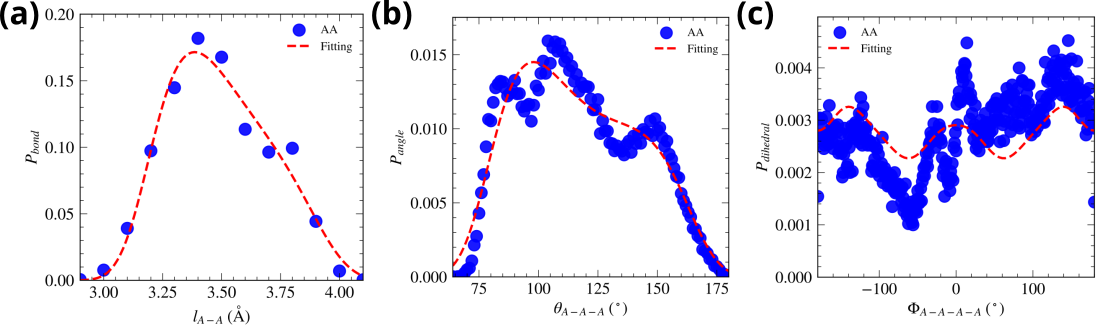
\includegraphics[width = 0.9\textwidth]{figs/ass1_probs.png}
    \caption{The results of a single iteration of Boltzmann inversion for (a) the bond distance (b) the bond angle and (c) the dihedrals. The resepective fits correspond to the interaction potentials described earlier in the text. The resulting final bonded interaction is given in equation \eqref{eq:ass1_final_bondendEng}.}
    \label{fig:ass1_distribs}
  \end{figure}

  The single-iteration Boltzmann inversion results in a final bonded interaction between CG beads of
  \begin{equation}
    \begin{split}
      E_\text{bonded} &= K_{r,2}(r - r_0)^2 +   K_{r,3}(r - r_0)^3 +  K_{r,4}(r - r_0)^4 \\
                      &~+ K_{\theta,2}(\theta - \theta_0)^2 +   K_{\theta,3}(\theta - \theta_0)^3 +  K_{\theta,4}(\theta - \theta_0)^4  \\
                      &~~+ \sum_{i=1}^7 A_i \cos^{i-1}(\phi),
    \end{split}
    \label{eq:ass1_final_bondendEng}
  \end{equation}
  with coefficients
  \begin{align*}
    \bm{E}&_\textbf{bond}: && r_0 =  3.38588 \text{\AA} && K_{r,i} = \{5.99659, -16.18383, 19.99841\}\text{kcal/mol} \\
    \bm{E}&_\textbf{angle}: && \theta_0 =  97.910908 ^\circ&& K_{\theta,i} = \{2.02467, -3.79927, 2.17714\}\text{kcal/mol} \\
    \bm{E}&_\textbf{dihed}: && && A_i = \{3.55479, 0.22113, 0.01174, -0.15241, -0.37184, -0.07968, 0.29841\}\text{kcal/mol}
  \end{align*}



\newpage
\section{Assignment 2: Walking Randomly}
\subsection{Theoretical Scaling Law}
One of the fundamental concepts of polymer physics is that of scaling laws, which aim to describe interactions in the context of different length scales.
The key length scale is that at which the interaction energy is comparable to that of the thermal energy $k_BT$. 
For scales smaller than this, the interactions of the polymer are dominated by the thermal energy and thus behave according to unperturbed statistics, while for larger length scales the polymer conformations are dominated by the interactions.

In the case of single chain conformations in solvents, the interaction of interest is that of the excluded volume interaction. For good solvents, the excluded volume interaction is positive, i.e., interaction with the solvent is more favorable than with itself, allowing for the chain to be more extended. On the other hand, poor solvents are described by a negative excluded volume interaction in which the polymer tends to collapse in on itself due to the unfavorable interactions with the solvent. The dependence of the size of a polymer chain on the number of monomers $N \gg 1$ can be described for both good and poor solvents by a power law:
\begin{equation}
  R \approx b N^\nu,
\end{equation}
where $\nu \approx 3/5$ for good solvents and $\nu = 1/3$ in poor solvents \cite{rubinsteinPolymerPhysics2003}. 

\subsection{Model and Results}
The environment of a good and poor solvents was implemented implicitly through the use of a modified Lennord-Jones potential between monomer beads:
\begin{equation}
  E_\text{LJ} = 4 \varepsilon \left[\left(\frac{\sigma}{r}\right)^{12} - \left(\frac{\sigma}{r}^{6}\right)\right], ~~ r < r_c,
\end{equation}
where $\varepsilon$ represents the strength of the interaction, $\sigma$ the zero-crossing distance, and $r_c$ the cut-off distance. 
Following Chang and Yethiraj \cite{Chang_LJ}, both solvents had the same strength of $\varepsilon = 1$ and zero-crossing of $\sigma = 1.0$ while the quality of solvent was induced through the cut-off of the potential. 
The good solvent was implemented through a purely repulsive potential with $r_c = 1.12246 \approx 2 ^{1/6}$ while a "full" LJ potential was used for the poor solvent with $r_c =  2.5$. 

Figure \ref{fig:ass2_rgs} shows that this implementation is in good agreement with the theoretical scaling arguments. The relatively large error bars are due to the value of $R_g$ being taken as the average throughout the entire simulation of the single chain. 
\begin{figure}[h]
  \centering  
  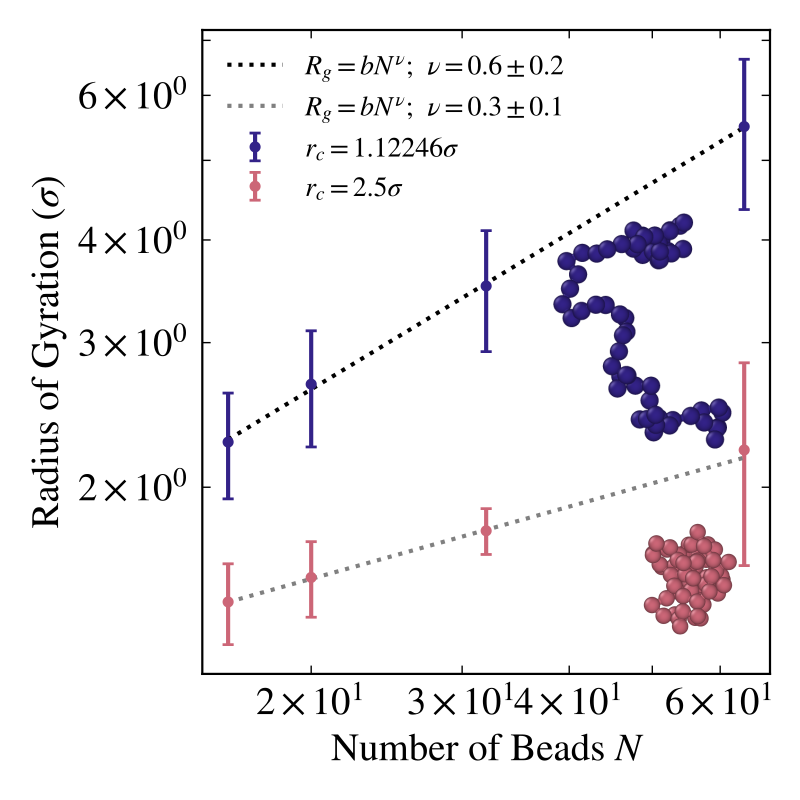
\includegraphics[width = 0.45\textwidth]{figs/ass2_rgs.png}
  \caption{The radius of gyration $R_g$ of a single polymer chain with $N = \{16, 20, 32, 64\}$ monomers in both good (blue) and poor (red) solvent conditions. The values of $R_g$ and the error were determined by taking average standard deviation, respectively, over the entire trajectory. The insets show the final conformation of a $N=64$ chain in good (blue) and poor (red) solvent conditions. }
  \label{fig:ass2_rgs}
\end{figure}

\newpage
\section{Assignment 3: Digital Breaking Bad}
\subsection{Digital Synthesis using create\_polymer.py}
Through the use of the \texttt{create\_polymer.py} script, several types of block grafted polymers of many atom types can be synthesized. Mainly, the length of the backbone, the length of the side chains, the frequency of grafting side chains, and the sequence ('AA', 'AB', 'ABA', etc.) for the backbone types. 
The script applies an equal amount of each atom type in the sequence, however, changing the block percentage can be achieved by repeating an atom type in the sequence e.g.,  'ABBB'. Figure \ref{fig:ass3_testTopos} show several examples of polymers created using this script.

\begin{figure}[h]
  \centering  
  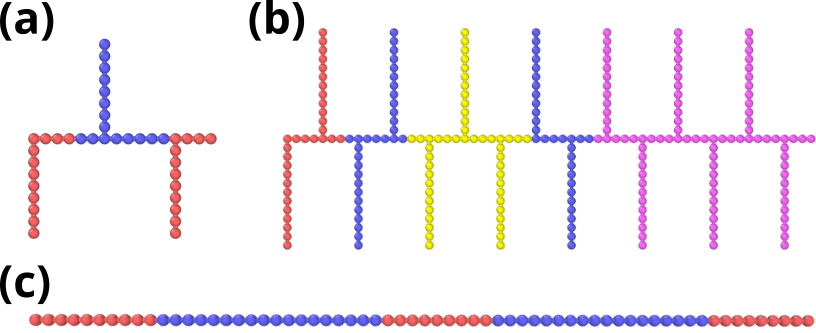
\includegraphics[width = 0.8\textwidth]{figs/ass3_test-topos.png}
  \caption{Example of different polymers "synthesized" using the \texttt{create\_polymer.py} script. \textbf{(a)} A grafted block polymer with backbone length of 16 with  sidechains of length 8 grafted every 5 beads of sequence 'ABBA'. \textbf{(b)} A different grafted polymer with backbone length of 60  grafted with sidechains of length 12 every 4 beads with block sequence 'ABCCBDDD'.  \textbf{(c)} a linear block polymer with backbone length 64 with block sequence of 'ABBABBA'. It is noted that polymers (a) and (c) have equal molecular weight of 64.}
  \label{fig:ass3_testTopos}
\end{figure}

Due to the proximity and relative short length of the two "A" blocks in polymer of Figure \ref{fig:ass3_testTopos}(a), one can expect the polymers to self-assemble into micelles with the hydrophobic A blocks at the core and the hydrophilic B block as the arms. Similar behavior can be expected for the linear block polymer in Figure \ref{fig:ass3_testTopos}(b). The self-assembly behavior of the polymer Figure \ref{fig:ass3_testTopos}(b) is difficult to intuitively predict. Nonetheless, if the self-interaction of the D blocks if favorable, self-assembly of micelle structures is expected due to the large percentage of the D block compared to the rest.  

\subsection{Setting of Interactions and Equlibration}
The polymers of Figure \ref{fig:ass3_testTopos}(a) and Figure \ref{fig:ass3_testTopos}(c) were simulated with good solvent conditions for the "B" (blue) block and poor solvent conditions for the "A" (red) block. This was implemented in the same manner as Assignment 2. The inter-block interaction was additionally set to be self-avoiding using the same interaction as block "B", as shown in Listing \ref{lst:ass3_interactions}. 
\begin{lstlisting}[language=Python, label=lst:ass3_interactions,
    caption={The interactions between the two blocks of the simulated linear and grafted polymers, Figure \ref{fig:ass3_testTopos}(a) and Figure \ref{fig:ass3_testTopos}(c) respectively.}
    ]
pair_style      lj/cut 2.5
pair_coeff      1  1  1.0  1.0  2.5
pair_coeff      1  2  1.0  1.0  1.14556
pair_coeff      2  2  1.0  1.0  1.14226
\end{lstlisting}

The simulation of each polymer type consisted of 150 polymers at a packing fraction of approximately 20\%. This was done to achieve relatively good statistics as well to avoid too long equilibration. Equilibration was achieved for both polymer solutions as can be seen in Figure \ref{fig:ass3_equilib}. It is noted that the runtime of the grafted polymer was reduced due to the quick equilibration of the linear polymer, however a longer run would better demonstrate that equilibrium was reached. 
\begin{figure}[h]
  \centering  
  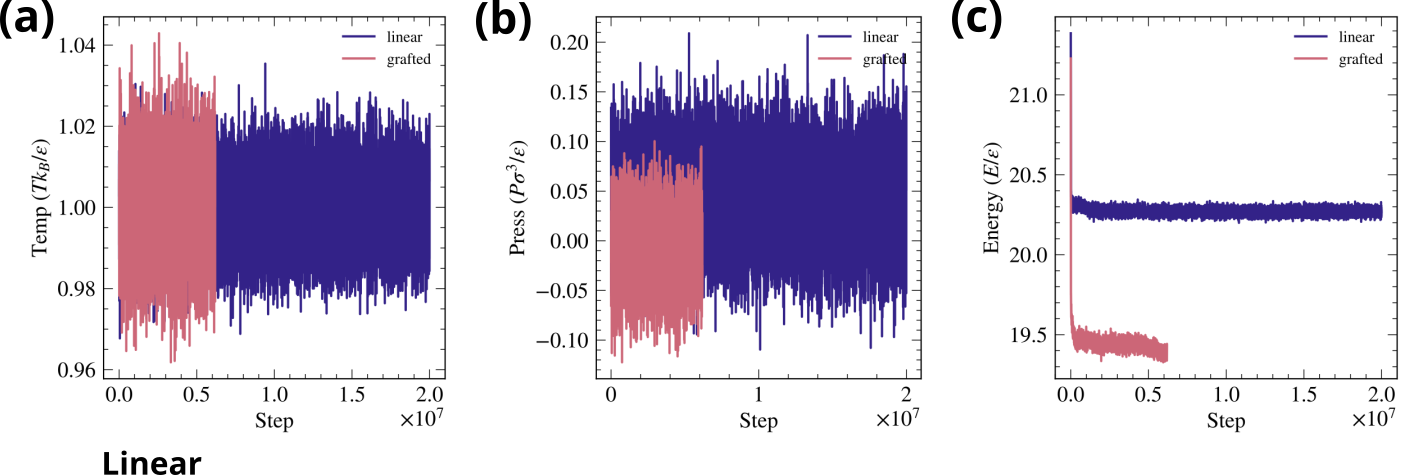
\includegraphics[width = 0.95\textwidth]{figs/ass3_equilib.png}
  \caption{The thermodynamic properties, (a) temperature (b) pressure (c) total energy, plotted against the simulation steps as to demonstrate equilibrium.}
  \label{fig:ass3_equilib}
\end{figure}

\newpage
\subsection{Results}
\texttt{Ovito} visualizations of the final assembled structures for the grafted and linear polymers are shown in Figure \ref{fig:ass3_assembled}.
The visualizations show that the both the linear and grafted polymer form micelle-like structures, with hydrophobic cores. However, with the linear architecture, there seems to be a connection between micellular structures, leading to a percolated assembly, which is not observed with the grafted structure. This is possibly due to the larger separation of the hydrophobic blocks by hydrophilic blocks within the polymer, which allow a single polymer chain to span multiple hydrophobic cores. However, I did not find a way to implement a quantitative analysis of this hypothesis. Moreover, visually, the characteristic size of the formed structures for both simulations is comparable to the simulation box, which can lead to finite size effects influencing the interactions. Simulation at a larger box size, but same concentration could elucidate whether finite size effects influenced the current simulation. 
\begin{figure}[h]
  \centering  
  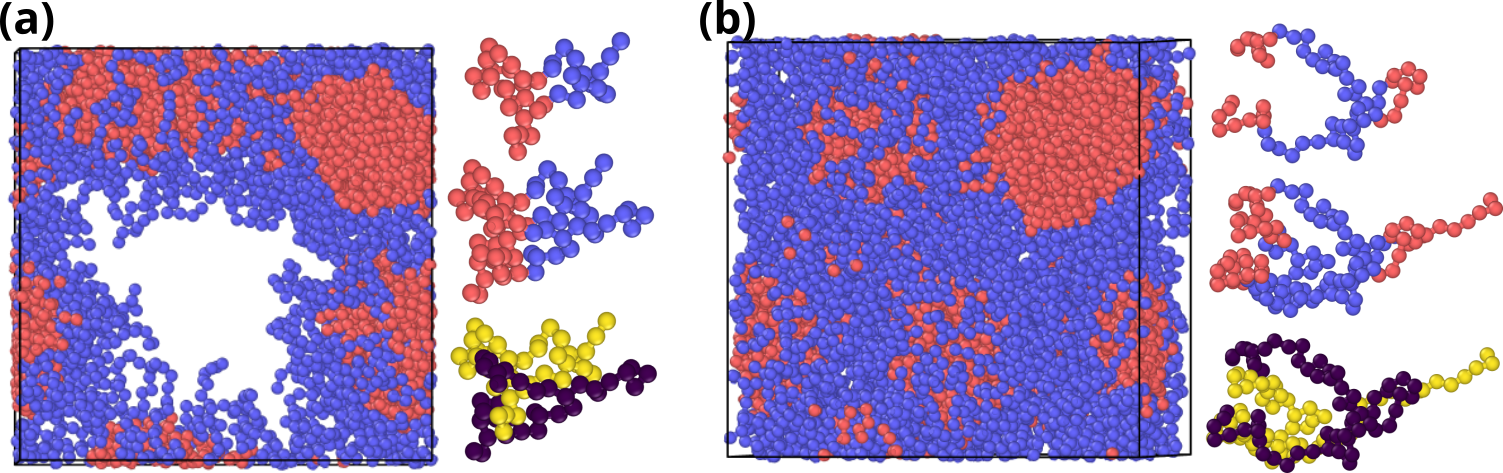
\includegraphics[width = 0.95\textwidth]{figs/ass3_assembled.png}
  \caption{\texttt{Ovito} visualizations of the final assembled structures for (a) the grafted polymer solution and (b) the linear polymer solution.  The left figure shows  the entire final assembled ensemble. The right shows a single selected polymer (top), with one of its neighboring polymers (middle), and the same two polymers, but with each polymer shown with a different color (bottom). The grafted polymer solution tends to form isolated micelles with minimal interconnectivity, while the linear polymer solution seems to show more percolation.}
  \label{fig:ass3_assembled}
\end{figure}

\newpage
\section{Assignment 4: Opposites Attract}
\subsection{Model Information}
Figure \ref{fig:ass4_equlib} shows the initial equilibrated data of the complex coacervate with zero salt. 
The complex coacervate consists of and equal amount of positive and negative linear polyelectrolytes with a total of 100 polyelectrolytes. Each polyelectrolyte consists of 50 beads with each bead having a charge magnitude of $1q/\sqrt{4\pi\epsilon_0\sigma\epsilon}$. The non-bonded interactions between particles are governed by the \texttt{lj/cut/coul/long} pair style of LAMMPS with a LJ cutoff of 1.12 and a Coulomb cutoff of 8.0. The average size of the polyelectrolytes is $R_g = (2.7 \pm 0.4) \sigma$, while the simulation box dimensions are $x, y, z = (15, 100, 15) \sigma$. As the sum of the average polymer size and Coulomb cutoff is less than the length of the simulation size, finite size effects are not likely. 
\begin{figure}[h]
  \centering  
  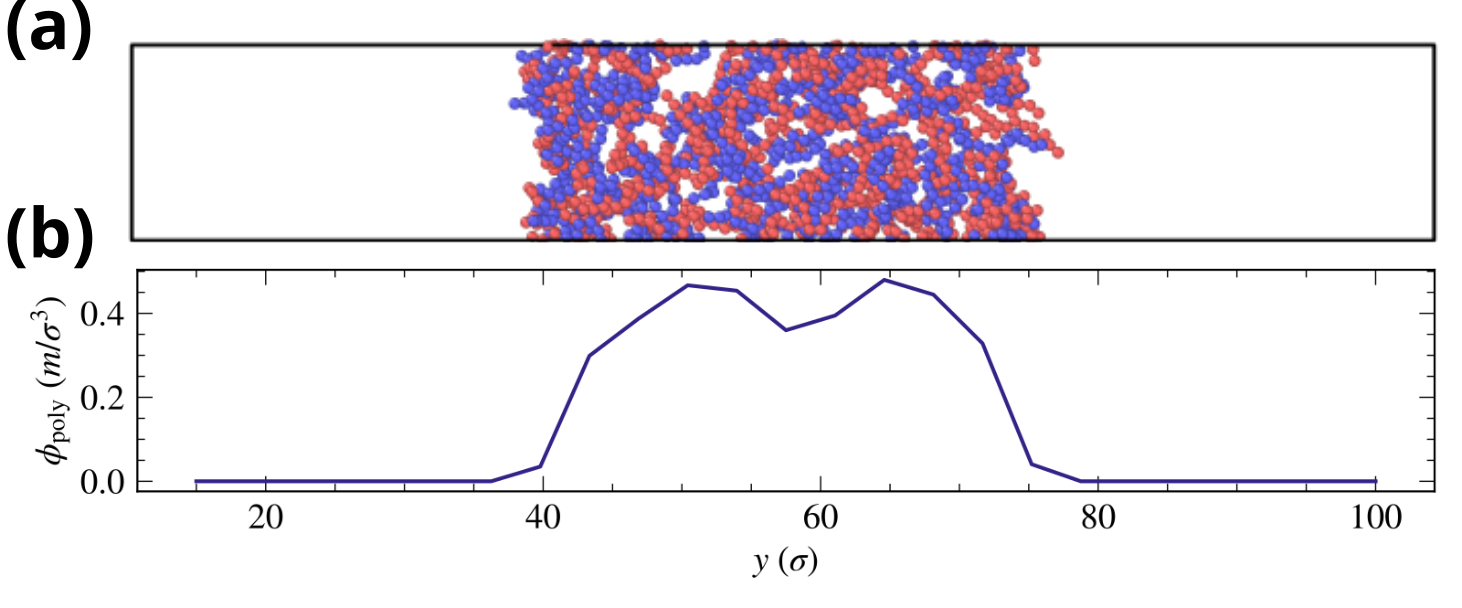
\includegraphics[width = 0.65\textwidth]{figs/ass4_equilib.png}
  \caption{(a) \texttt{Ovito} visualization of the equilibrated structures and (b) the linear mass density of the polyelectrolytes with no added salt. The red polymers represent the positive polyelectrolytes, while the blue represent the negative polyelectrolytes.}
  \label{fig:ass4_equlib}
\end{figure}

\subsection{Binodal Curve}
To determine the binodal curve of the complex coacervation process, the bulk salt density $\phi_\text{bulk}$ was simulated in a range of 0.09 to 0.31 $m/\sigma^3$. This was done by keeping the volume constant, but varying the number of salt particles from 2000 to 7000 in steps of 1000. Each bulk salt concentration was simulated for 1000000 steps, with frames being saved every 1000 steps.  The polymer-dense coacervate and supernatant phase were defined using the linear density profiles along the  y-axis following \cite{Nayan}. Mainly, the polymer-dense coacervate was defined as the regions where the polyelectrolyte density is within 20\% of the maximum polyelectrolyte density while the supernatant phase was defined as the regions where the polyelectrolyte density is less than 20\% of the maximum  polyelectrolyte density.  From the spinodal curve, the critical salt concentration is expected to be around 0.6 $m/\sigma^3$. 

\begin{figure}[h]
  \centering  
  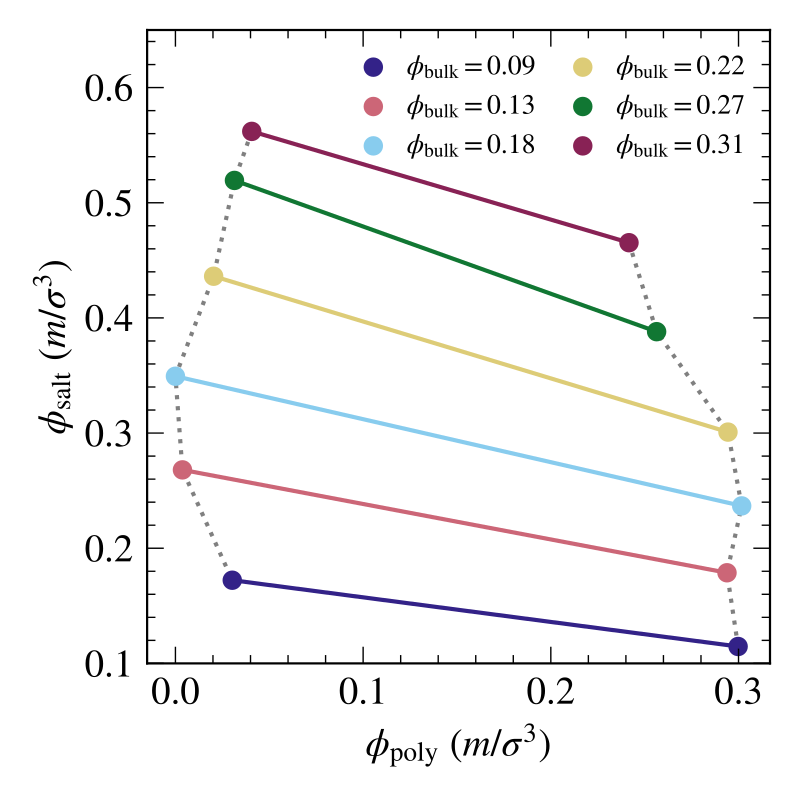
\includegraphics[width = 0.4\textwidth]{figs/ass4_binodalcurve.png}
  \caption{The resulting binodal curve from the simulations with varying bulk salt concentration. The left points are determined from salt and polymer density in the supernatent phase, while the right points are determined from the respective densities in the coacervate phase. }
  \label{fig:ass4_equlib}
\end{figure}

\printbibliography

% \begin{appendices}
%   \input{Appendix}
% \end{appendices}

\end{document}



